\documentclass{article} % say
\usepackage{tikz}
\begin{document}
We are working on
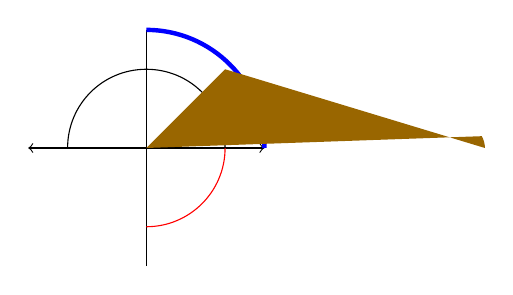
\begin{tikzpicture}
\draw[<->] (-1.5,0) -- (1.5,0);
\draw (0,-1.5) -- (0,1.5);
\draw (-1,0) .. controls (-1,0.555) and (-0.555,1) .. (0,1)
.. controls (0.555,1) and (1,0.555) .. (1,0);
\draw[red] (1,0) arc [start angle=0, end angle=-90, radius=1cm];
\draw[blue,ultra thick] (0,1.5) arc [start angle=90, end angle=0, radius=1.5cm];
\fill[green!40!red] (1,1) -- (43mm,0mm)
arc [start angle=0, end angle=30, radius=3mm] -- (0,0);
\end{tikzpicture}

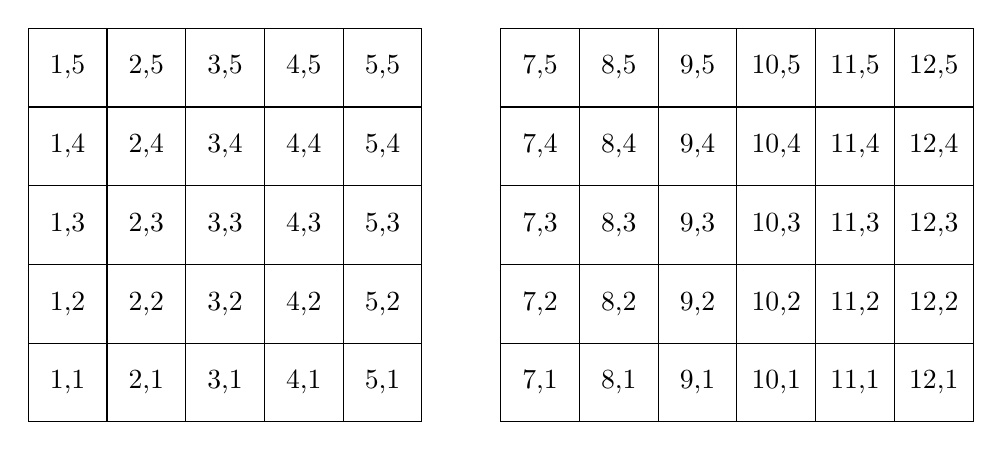
\begin{tikzpicture}
\foreach \x in {1,2,...,5,7,8,...,12}
\foreach \y in {1,...,5}
{
\draw (\x,\y) +(-.5,-.5) rectangle ++(.5,.5);
\draw (\x,\y) node{\x,\y};
}
\end{tikzpicture}
\end{document}